\section{Creación de una Dimensión Regular}  

1. En el Solution Explorer nos ubicamos en Data Sources View y podemos ver que tenemos la vista de las
siguientes tablas:
	\begin{center}
	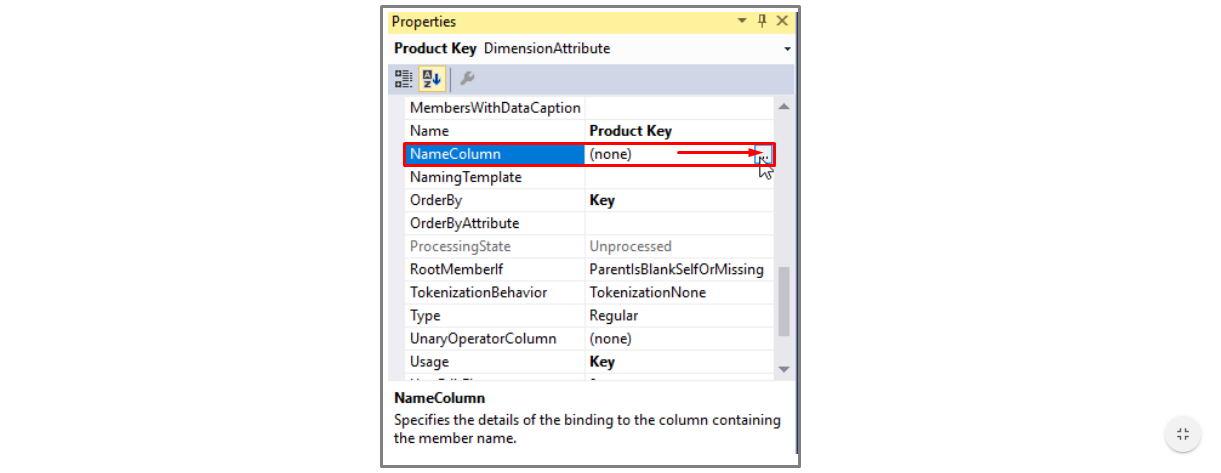
\includegraphics[width=\columnwidth]{images/task1/img1}
	\end{center}	


2. Siempre se recomienda primero crear las dimensiones y como paso final recién crear el cubo, es por eso que
eliminamos el cubo creado en el primer post. Luego nos dirigimos a Dimensions. Click derecho y ubicamos
New Dimension
	\begin{center}
	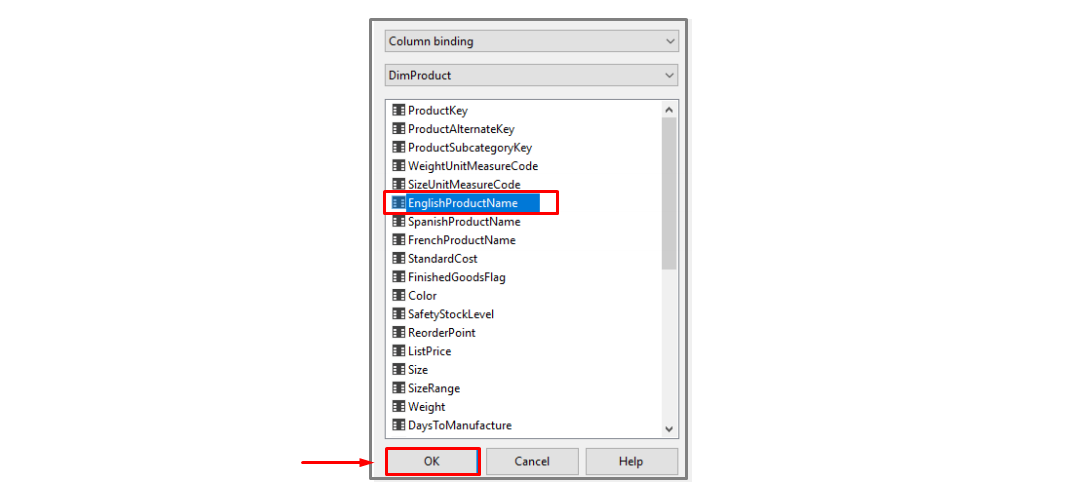
\includegraphics[width=\columnwidth]{images/task1/img2}
	\end{center}	

3. Nos abrirá un Wizard, donde la primera ventana es un resumen de lo que se puede realizar.
	\begin{center}
	
\includegraphics[width=\columnwidth]{images/task1/img3}
	\end{center}	

4. Click en Next.
Esta paso en el wizard es muy importante ya que nos permite seleccionar el origen de la dimensión a crear.
Se tienen 4 opciones:
			\begin{itemize}
				\item Use an existing table: Se seleccionará alguna tabla perteneciente al Data Source View.
				\item Generate a time table in the data source: Crea una tabla en el data source, pero esta nueva tabla no
es replicada en el origen.
\item Generate a time table in the server: Crea una tabla en el server, y esta nueva tabla es replicada en
el origen.
\item Generate a non table in the data source: Crea una tabla en el data source a partir de unos
Templates que tiene el Data Tools.

Seleccionamos la primera opcion:

			\end{itemize}

	\begin{center}
	
\includegraphics[width=\columnwidth]{images/task1/img4}
    \end{center}	

5. Click en Next.
Seleccionamos el Data source view (podríamos tener más de uno) y la tabla Dimensión, en este ejemplo
DimProduct. En Key columns por defecto siempre selecciona al Primary Key de la tabla, pero este valor luego
podría ser cambiado. También podemos añadirle un Name Column a este Key column pero lo dejaremos tal
como esta:
    
	\begin{center}
	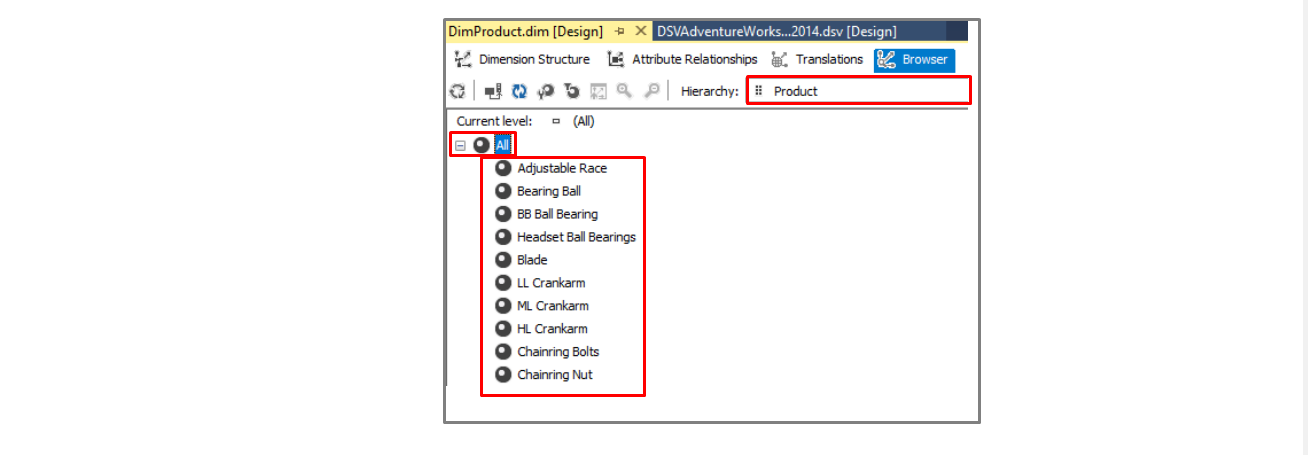
\includegraphics[width=\columnwidth]{images/task1/img5}
    \end{center}	

6. Click en Next.
Marcamos los atributos con los cuales trabajaremos:
    
	\begin{center}
	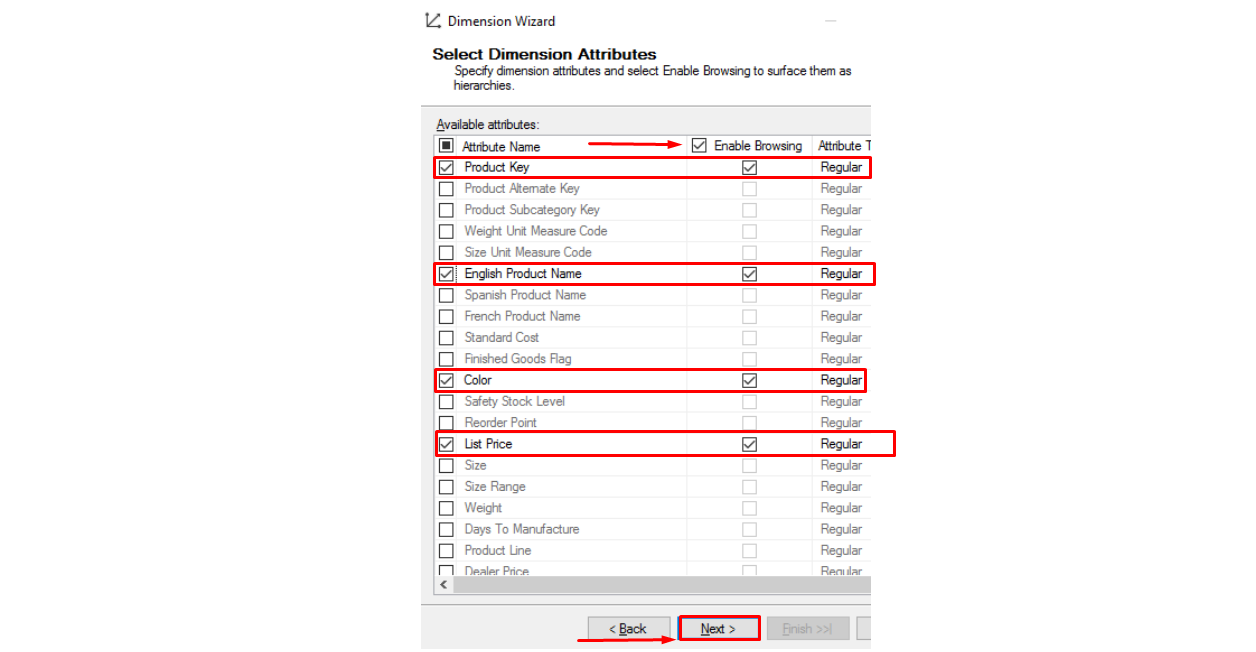
\includegraphics[width=\columnwidth]{images/task1/img6}
    \end{center}	

7. Click en Next.
Indicamos el Nombre a la dimensión:
    
	\begin{center}
	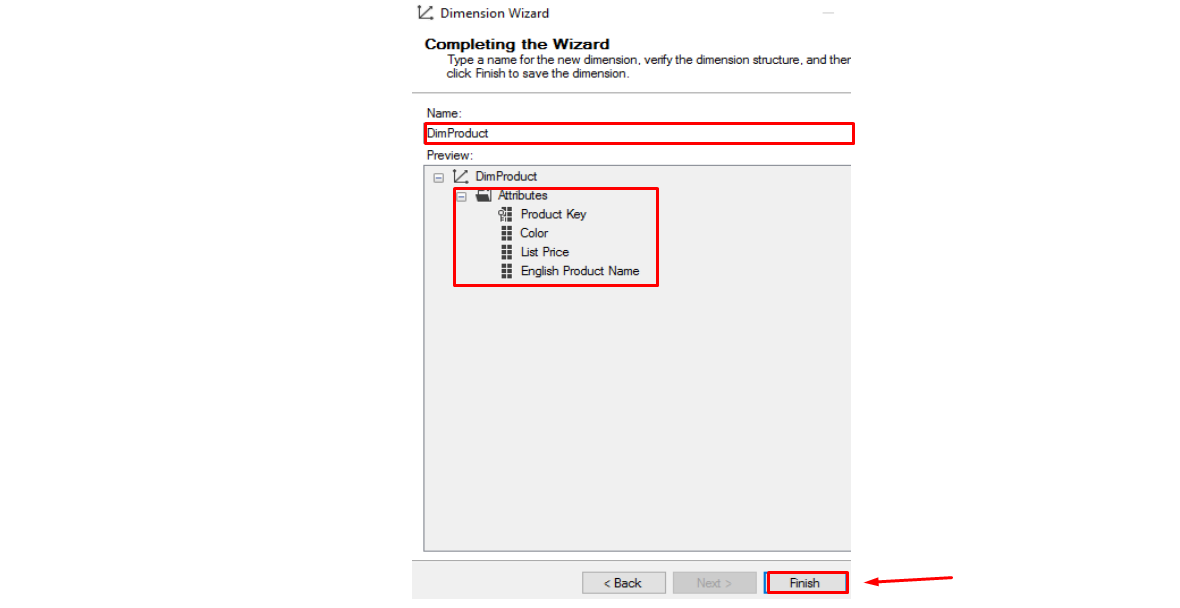
\includegraphics[width=\columnwidth]{images/task1/img7}
    \end{center}	

Click en Finish.

    